
\chapter{확률밀도함수}
\label{density}
\index{PDF}
\index{확률밀도함수 (probability density function)}
\index{지수분포 (exponential distribution)}
\index{분포 (distribution)!지수 (exponential)}
\index{정규분포 (normal distribution)}
\index{분포 (distribution)!정규 (normal)}
\index{가우스 분포 (Gaussian distribution)}
\index{분포 (distribution)!가우스 (Gaussian)}
\index{CDF}
\index{미분 (derivative)}


이번 장에서 사용되는 코드는 {\tt density.py}에 있다.
코드를 다운로드하고 작업하는 것에 대한 정보는 ~\ref{code}을 참조한다.

\section{PDF}

CDF 미분을 {\bf 확률밀도함수 (probability density function)}, PDF라고 한다.
예를 들어, 지수분포 PDF는 다음과 같다.

%
\[ \PDF_{expo}(x) = \lambda e^{-\lambda x}   \]
%
정규분포 PDF는 다음과 같다.
%
\[ \PDF_{normal}(x) = \frac{1}{\sigma \sqrt{2 \pi}} 
                 \exp \left[ -\frac{1}{2} 
                 \left( \frac{x - \mu}{\sigma} \right)^2 \right]  \]
%

$x$ 특정한 값에 대한 PDF를 계산하는 것이 대체로 유용하지는 않다. 결과가 확률이 아니기 때문이다; 확률 {\em 밀도 (density)}다.
\index{밀도 (density)}
\index{질량 (mass)}

물리학에서 밀도는 단위 체적당 질량이다; 질량을 계산하려면, 체적을 곱하거나 혹은 만약 밀도가 상수가 아니라면 체적에 대해 적분해야 한다.

마찬가지로, {\bf 확률 밀도 (probability density)}는 단위 $x$당 확률을 측정한다. 확률 질량을 계산하려면, $x$에 대해서 적분해야 한다. 

{\tt thinkstats2}는 Pdf라는 클래스로 확률밀도함수를 나타낸다.
모든 Pdf 객체는 다음 메쏘드를 제공한다:

\begin{itemize}

\item {\tt Density}, {\tt x}를 인자로 받아 {\tt x}에서 분포 밀도를 반환한다.

\item {\tt Render}는 이산 집합값 대해 밀도를 평가하고 시퀀스 짝을 반환한다: 정렬된 {\tt xs}과 상응하는 확률 밀도{\tt ds}.

\item {\tt MakePmf}, 이산 집합값에 대해 {\tt Density}를 평가하고 Pdf에 그사하는 정규화된 Pmf를 반환한다.
\index{Pmf}

\item {\tt GetLinspace}, {\tt Render}와 {\tt MakePmf}에서 사용되는 기본설정 집합 점(point)을 반환한다.

\end{itemize}  

Pdf는 추상화된 부모 클래스로 의미하는 것은 인스턴스화하면 안된다; 즉, Pdf 객체를 생성할 수 없다. 대신에 Pdf를 상속받아 {\tt Density}과 {\tt GetLinspace} 정의하는 자식 클래스를 정의해야 한다. 
Pdf는 {\tt Render}과 {\tt MakePmf}을 제공한다.

예를 들어, {\tt thinkstats2}는 정규밀도함수를 평가하는 {\tt NormalPdf}라는 이름의 클래스를 제공한다.

\begin{verbatim}
class NormalPdf(Pdf):

    def __init__(self, mu=0, sigma=1, label=''):
        self.mu = mu
        self.sigma = sigma
        self.label = label

    def Density(self, xs):
        return scipy.stats.norm.pdf(xs, self.mu, self.sigma)

    def GetLinspace(self):
        low, high = self.mu-3*self.sigma, self.mu+3*self.sigma
        return np.linspace(low, high, 101)
\end{verbatim}

NormalPdf 객체는 모수 {\tt mu}과 {\tt sigma}을 담고 있다.
{\tt Density}는 {\tt scipy.stats.norm}을 사용하는데 정규분포를 표현한고, 
다른 메쏘드와 더불어 {\tt cdf}와 {\tt pdf}를 제공한다.(~\ref{normal}절 참조).
\index{SciPy}

다음 예제는 BRFSS에 있는 성인여성신장(cm 단위) 평균과 분산으로 NormalPdf를 생성한다(~\ref{brfss}절 참조). 그리고 나서, 평균에서 1 표준편차 지점에 분포 밀도를 계산한다.
\index{표준 편차 (standard deviation)}

\begin{verbatim}
>>> mean, var = 163, 52.8
>>> std = math.sqrt(var)
>>> pdf = thinkstats2.NormalPdf(mean, std)
>>> pdf.Density(mean + std)
0.0333001
\end{verbatim}

결과는 cm 당 확률질량 단위로 약 0.03이다.
한번더, 확률밀도는 그 자체로 의미는 없다. 하지만, Pdf를 플롯으로 그린다면, 분포 형상을 볼 수 있다.

\begin{verbatim}
>>> thinkplot.Pdf(pdf, label='normal')
>>> thinkplot.Show()
\end{verbatim}

{\tt thinkplot.Pdf}은 평활 함수(smooth function)로 Pdf 플롯을 그린다. 
계단함수로 Pmf을 그리는 {\tt thinkplot.Pmf}와 대조된다.
그림~\ref{pdf_example}에 결과가 있다. 다음 절에서 살펴볼 표본에서 추정한 PDF로 함께 플롯되어 그려져 있다.
\index{thinkplot}

Pdf를 근사하는데 {\tt MakePmf}를 사용할 수도 있다.

\begin{verbatim}
>>> pmf = pdf.MakePmf()
\end{verbatim}

기본설정으로, {\tt mu - 3*sigma}에서 {\tt mu + 3*sigma} 사이에 동일 간격을 지닌 101 점이 Pmf에 있다.
선택사양으로 {\tt MakePmf}와 {\tt Render}는 키워드 인자로 {\tt low}, {\tt high}, {\tt n}을 갖는다.

\begin{figure}
% pdf_example.py
%\centerline{\includegraphics[height=2.2in]{figs/pdf_example.pdf}}
\caption{A normal PDF that models adult female height in the U.S.,
and the kernel density estimate of a sample with $n=500$.}
\label{pdf_example}
\end{figure}


\section{핵밀도추정 (Kernel density estimation)} 

{\bf 핵밀도추정 (Kernel density estimation,KDE)}은
표본을 받아 데이터에 적합하는 적절한 평활 PDF를 찾는 알고리즘이다.
\url{http://en.wikipedia.org/wiki/Kernel_density_estimation}  웹사이트에서 좀더 자세한 정보를 얻을 수 있다.

\index{KDE}
\index{핵밀도추정 (kernel density estimation)}

{\tt scipy}에 KDE 구현된 것이 있고, 
{\tt thinkstats2}는 이를 사용해서 {\tt EstimatedPdf}라는 클래스를 제공한다.
\index{사이파이 (SciPy)}
\index{넘파이 (NumPy)}

\begin{verbatim}
class EstimatedPdf(Pdf):

    def __init__(self, sample):
        self.kde = scipy.stats.gaussian_kde(sample)

    def Density(self, xs):
        return self.kde.evaluate(xs)
\end{verbatim}

\verb"__init__"이 표본을 인자로 받아 핵밀도추정값을 계산한다.
결과는 \verb"gaussian_kde" 객체고 {\tt evaluate} 메쏘드를 제공한다.

{\tt Density}가 값 혹은 시퀀스를 인자로 받아 
\verb"gaussian_kde.evaluate"을 호출하고 결과 밀도를 반환한다.
단어 ``가우스 (Gaussian)''가 나오는데 이유는 KDE를 평활하는데 가우스 분포에 기반한 필터를 사용하기 때문이다.
\index{밀도 (density)}

다음에 정규분포에서 표본을 생성하고 표본에 적합하기 위해서 EstimatedPdf를 만드는 예제가 있다.
\index{넘파이 (NumPy)}
\index{EstimatedPdf}

\begin{verbatim}
>>> sample = [random.gauss(mean, std) for i in range(500)]
>>> sample_pdf = thinkstats2.EstimatedPdf(sample)
>>> thinkplot.Pdf(sample_pdf, label='sample KDE')
\end{verbatim}

\verb"sample"은 무작위 신장 500개 리스트다. 
\verb"sample_pdf"는 Pdf 객체로 추정된 KDE 표본정보를 담고 있다.
동일 간격 값의 시퀀스에서 밀도를 평가함으로써 {\tt pmf}는 Pmf 객체로 Pdf를 근사한다.

그림~\ref{pdf_example}에 정규밀도함수와 무작위 신장 500개 표본에 기반한 KDE가 있다. 추정값이 원분포에 좋은 매칭이다.

KDE로 밀도함수를 추정하는 것은 몇가지 목적으로 유용한다. 

\index{thinkplot}
\index{Pmf}

\begin{itemize}

\item {\it 시각화 (Visualization):} 
  프로젝트 탐색단계에서, CDF가 대체로 분포를 가장 잘 시각화한다.
  CDF를 살펴본 후에, 추정 PDF가 분포에 대한 적절한 모형인지 결정할 수 있다.
  만약 그렇다면, CDF에 익숙하지 않은 관계에게 분포를 제시하는데 더 좋은 선택지가 될 수 있다.
\index{시각화 (visualization)}
\index{모형 (model)}

\item {\it 보간 (Interpolation):} 
  추정 PDF는 표본에서 모집단 모형으로 가는 한 방법이다.
  만약 모집단 분포가 매끄럽다고 믿을 이유가 있다면, KDE를 사용해서 표본에 없는 값에 대해 밀도를 보간한다.
\index{보간 (interpolation)}

\item {\it 모의실험 (Simulation):} 
  모의실험은 종종 표본 분포에 기반한다. 
  만약 표본크기가 작다면, KDE를 사용해서 표본분포를 평활하는 것이 적절하다.
  관측점을 중복하기 보다 KDE가 모의실험을 통해서 좀더 가능한 결과값을 탐색하도록 한다.
\index{모의실험 (simulation)}

\end{itemize}


\section{분포 프레임워크 (distribution framework)}
\index{분포 프레임워크 (distribution framework)}

\begin{figure}
\centerline{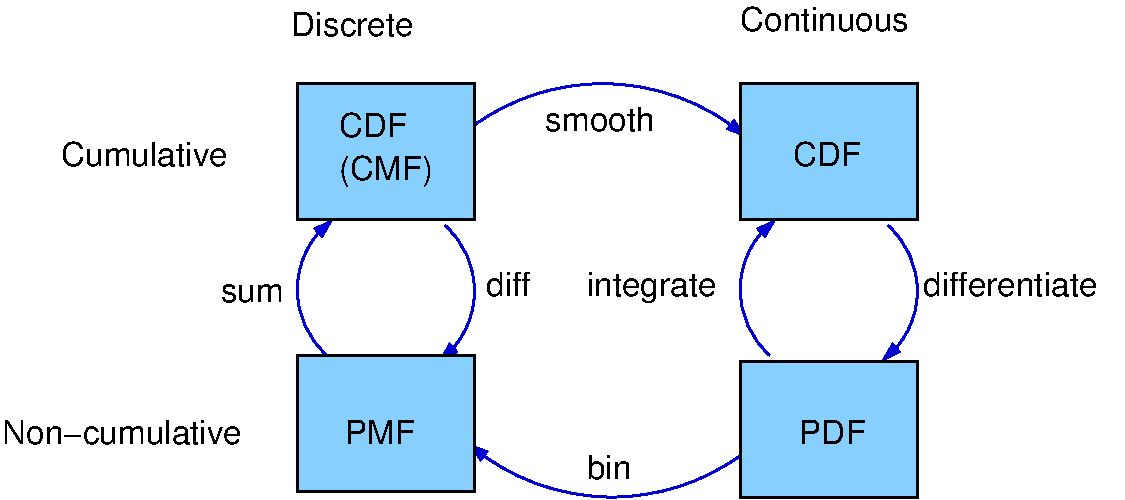
\includegraphics[height=2.2in]{figs/distribution_functions.pdf}}
\caption{A framework that relates representations of distribution
functions.}
\label{dist_framework}
\end{figure}

현재까지 PMF, CDF, PDF를 살펴봤다; 잠시 복습 시간을 가져본다.
그림~\ref{dist_framework}에 함수가 어떻게 서로 연관되는지 나타나 있다.
\index{Pmf}
\index{Cdf}
\index{Pdf}

PMF로 시작했는데, PMF는 이산 집합 값에 대한 확률을 나타낸다.
PMF에서 CDF를 얻기 위해서는, 확률 질량을 더해서 누적 확률을 얻는다.
CDF에서 PMF로 돌아가기 위해서는, 누적 확률 차이를 계산한다.
다음 몇 절에 걸쳐 이와 같은 연산을 어떻게 구현했는지 살펴볼 것이다.
\index{누적 확률 (cumulative probability)}

PDF는 연속형 CDF 미분이다; 혹은, 동등하게 CDF는 PDF의 적분이다.
PDF는 값을 확률 밀도로 매핑한다는 것을 기억하라; 확률값을 얻기 위해서,
적분해야 한다.

\index{이산 분포 (discrete distribution)}
\index{연속 분포 (continuous distribution)}
\index{평활 (smoothing)}

이산형에서 연속 분포를 얻기 위해서, 다양한 평활(smoothing) 작업을 수행할 수 있다.
평활의 한 형태는 데이터가 (지수 혹은 정규 분포처럼) 
해석 연속 분포(analytic continuous distribution)에서 왔다고 가정하는 것이다.
또 다른 선택 옵션은 핵밀도추정(kernel density estimation)이다.

\index{지수 분포 (exponential distribution)}
\index{분포 (distribution)!지수 (exponential)}
\index{정규 분포 (normal distribution)}
\index{분포 (distribution)!정규 (normal)}
\index{가우스 분포 (Gaussian distribution)}
\index{분포 (distribution)!가우스 (Gaussian)}

평활의 반대가 {\bf 이산화 (discretizing)}, 혹은 양자화(quantizing)다.
만약 이산 점에서 PDF를 평가한다면, PDF에 근사하는 PMF를 생성할 수 있다.
수치적분(numerical integration)을 사용해서 좀더 잘 근사할 수도 있다.
\index{이산화 (discretize)}
\index{양자화 (quantize)}
\index{구간화 (binning)}

연속CDF와 이산CDF를 구별하기 위해서, 이산CDF는 
``누적 질량 함수 (cumulative mass function)''가 되는 것이 좋을지도 모른다.
하지만, 저자가 알고 있는 바로는, 누구도 그 용어를 사용하지 않는다.
\index{CDF}



\section{Hist implementation}

At this point you should know how to use the basic types provided
by {\tt thinkstats2}: Hist, Pmf, Cdf, and Pdf.  The next few sections
provide details about how they are implemented.  This material
might help you use these classes more effectively, but it is not
strictly necessary.
\index{Hist}

Hist and Pmf inherit from a parent class called \verb"_DictWrapper".
The leading underscore indicates that this class is ``internal;'' that
is, it should not be used by code in other modules.  The name
indicates what it is: a dictionary wrapper.  Its primary attribute is
{\tt d}, the dictionary that maps from values to their frequencies.
\index{DictWrapper}
\index{internal class}
\index{wrapper}

The values can be any hashable type.  The frequencies should be integers,
but can be any numeric type.
\index{hashable}

\verb"_DictWrapper" contains methods appropriate for both
Hist and Pmf, including \verb"__init__", {\tt Values},
{\tt Items} and {\tt Render}.  It also provides modifier
methods {\tt Set}, {\tt Incr}, {\tt Mult}, and {\tt Remove}.  These
methods are all implemented with dictionary operations.  For example:
\index{dictionary}

\begin{verbatim}
# class _DictWrapper

    def Incr(self, x, term=1):
        self.d[x] = self.d.get(x, 0) + term

    def Mult(self, x, factor):
        self.d[x] = self.d.get(x, 0) * factor

    def Remove(self, x):
        del self.d[x]
\end{verbatim}

Hist also provides {\tt Freq}, which looks up the frequency
of a given value.
\index{frequency}

Because Hist operators and methods are based on dictionaries,
these methods are constant time operations;
that is, their run time does not increase as the Hist gets bigger.
\index{Hist}


\section{Pmf implementation}

Pmf and Hist are almost the same thing, except that a Pmf
maps values to floating-point probabilities, rather than integer
frequencies.  If the sum of the probabilities is 1, the Pmf is normalized.
\index{Pmf}

Pmf provides {\tt Normalize}, which computes the sum of the
probabilities and divides through by a factor:

\begin{verbatim}
# class Pmf

    def Normalize(self, fraction=1.0):
        total = self.Total()
        if total == 0.0:
            raise ValueError('Total probability is zero.')

        factor = float(fraction) / total
        for x in self.d:
            self.d[x] *= factor

        return total
\end{verbatim}

{\tt fraction} determines the sum of the probabilities after
normalizing; the default value is 1.  If the total probability is 0,
the Pmf cannot be normalized, so {\tt Normalize} raises {\tt
  ValueError}.

Hist and Pmf have the same constructor.  It can take
as an argument a {\tt dict}, Hist, Pmf or Cdf, a pandas
Series, a list of (value, frequency) pairs, or a sequence of values.
\index{Hist}

If you instantiate a Pmf, the result is normalized.  If you
instantiate a Hist, it is not.  To construct an unnormalized Pmf,
you can create an empty Pmf and modify it.  The Pmf modifiers do
not renormalize the Pmf.


\section{Cdf implementation}

A CDF maps from values to cumulative probabilities, so I could have
implemented Cdf as a \verb"_DictWrapper".  But the values in a CDF are
ordered and the values in a \verb"_DictWrapper" are not.  Also, it is
often useful to compute the inverse CDF; that is, the map from
cumulative probability to value.  So the implementaion I chose is two
sorted lists.  That way I can use binary search to do a forward or
inverse lookup in logarithmic time.
\index{Cdf}
\index{binary search}
\index{cumulative probability}
\index{DictWrapper}
\index{inverse CDF}
\index{CDF, inverse}

The Cdf constructor can take as a parameter a sequence of values
or a pandas Series, a dictionary that maps from values to
probabilities, a sequence of (value, probability) pairs, a Hist, Pmf,
or Cdf.  Or if it is given two parameters, it treats them as a sorted
sequence of values and the sequence of corresponding cumulative
probabilities.

Given a sequence, pandas Series, or dictionary, the constructor makes
a Hist.  Then it uses the Hist to initialize the attributes:

\begin{verbatim}
        self.xs, freqs = zip(*sorted(dw.Items()))
        self.ps = np.cumsum(freqs, dtype=np.float)
        self.ps /= self.ps[-1]
\end{verbatim}

{\tt xs} is the sorted list of values; {\tt freqs} is the list
of corresponding frequencies.  {\tt np.cumsum} computes
the cumulative sum of the frequencies.  Dividing through by the
total frequency yields cumulative probabilities.
For {\tt n} values, the time to construct the
Cdf is proportional to $n \log n$.
\index{frequency}

Here is the implementation of {\tt Prob}, which takes a value
and returns its cumulative probability: 

\begin{verbatim}
# class Cdf
    def Prob(self, x):
        if x < self.xs[0]:
            return 0.0
        index = bisect.bisect(self.xs, x)
        p = self.ps[index - 1]
        return p
\end{verbatim}

The {\tt bisect} module provides an implementation of binary search.
And here is the implementation of {\tt Value}, which takes a
cumulative probability and returns the corresponding value:

\begin{verbatim}
# class Cdf
    def Value(self, p):
        if p < 0 or p > 1:
            raise ValueError('p must be in range [0, 1]')

        index = bisect.bisect_left(self.ps, p)
        return self.xs[index]
\end{verbatim}

Given a Cdf, we can compute the Pmf by computing differences between
consecutive cumulative probabilities.  If you call the Cdf constructor
and pass a Pmf, it computes differences by calling {\tt Cdf.Items}:
\index{Pmf}
\index{Cdf}

\begin{verbatim}
# class Cdf
    def Items(self):
        a = self.ps
        b = np.roll(a, 1)
        b[0] = 0
        return zip(self.xs, a-b)
\end{verbatim}

{\tt np.roll} shifts the elements of {\tt a} to the right, and ``rolls''
the last one back to the beginning.  We replace the first element of
{\tt b} with 0 and then compute the difference {\tt a-b}.  The result
is a NumPy array of probabilities.
\index{NumPy}

Cdf provides {\tt Shift} and {\tt Scale}, which modify the
values in the Cdf, but the probabilities should be treated as
immutable.


\section{적률 (Moments)}
\index{적률 (moment)}

어느 때고 표본을 얻고 하나의 숫자로 줄일 수 있다. 그 숫자가 통계량(statistic)이다.
지금까지 살펴본 통계량은 평균, 분산, 중위수, 그리고 사분위수다.

{\bf 원적률 (raw moment)}은 일종의 통계량이다. 만약 $x_i$ 표본 값이 있다면,
$k$번째 원적률은 다음과 같다.

%
\[ m'_k = \frac{1}{n} \sum_i x_i^k \]
%
혹은, 파이썬 표기법으로 표현하면, 다음과 같다.

\begin{verbatim}
def RawMoment(xs, k):
    return sum(x**k for x in xs) / len(xs)
\end{verbatim}

$k=1$일 때, 결과는 표본 평균 $\xbar$가 된다.
다른 원적률은 그 자체로 의미가 있지 않다. 하지만, 다른 계산에 사용된다.

{\bf 중심적률(central moments)}이 더 유용하다. 
$k$번째 중심적률은 다음과 같다.
%
\[ m_k = \frac{1}{n} \sum_i (x_i - \xbar)^k \]
%

혹은 파이썬으로 표현하면 다음과 같다.

\begin{verbatim}
def CentralMoment(xs, k):
    mean = RawMoment(xs, 1)
    return sum((x - mean)**k for x in xs) / len(xs)
\end{verbatim}

$k=2$일 때, 결과는 두번째 중심 적률로 분산으로 인지하고 있을 것이다.
분산의 정의가 왜 이러한 통계량이 적률로 불리는지 힌트를 준다.
각 위치 $x_i$에 자를 따라 추를 달고 평균 주위에서 자를 돌리면, 
회전추의 관성 적률은 값의 분산이다. 만약 관성 적률에 익숙하지 않다면,
\url{http://en.wikipedia.org/wiki/Moment_of_inertia} 웹사이트를 참조한다.  
\index{관성 적률(moment of inertia)}

적률에 기반한 통계를 보고할 때, 단위(unit)에 관한 생각이 중요하다.
예를 들어, 값 $x_i$가 cm 이라면, 첫 원적률은 또한 cm이다.
하지만, 두번째 적률은 cm$^2$이고, 세번째 적률은 cm$^3$... 등등이 된다.

이러한 단위 때문에, 적률은 그 자체로 해석하기 어렵다.
두번째 적률에 대해서 분산에 제곱근을 취한 표준편차를 쓰는 것이 이러한 이유다. 
그러면 $x_i$와 단위가 같아진다.
\index{표준 편차 (standard deviation)}


\section{왜도 (Skewness)}
\index{왜도 (skewness)}

{\bf 왜도 (Skewness)}는 분포 형태를 기술하는 속성이다. 
만약 분포가 중심 경향성 주변에서 대칭이라면, 기울어지지 않았다.
만약 값들이 오른쪽으로 좀더 뻗어져 있다면, ``오른쪽으로 기울어져 (right
skewed)'' 있고, 만약 값들이 왼쪽으로 치우쳐 있다면, ``왼쪽으로 기울어져 (left
skewed''있다.

\index{중심 경향성 (central tendency)}

``기울어짐 (skewed)''을 사용하는 것다는 것이 ``편의(biased)''를 함축하지는 않는다.
단지 왜도는 분포 형태만을 기술한다; 표본 추출과정에 편의가 있는지에 관해 
어떤 것도 나타내지 않는다.

\index{편의 (bias)}
\index{표본 왜도 (sample skewness)}

흔히 몇몇 통계량이 분포 왜도를 계량화하는데 사용된다.
주어진 값 시퀀스가 $x_i$가 주어졌을 때, 
{\bf 표본 왜도 (sample skewness)} $g_1$은 다음과 같이 계산된다.

\begin{verbatim}
def StandardizedMoment(xs, k):
    var = CentralMoment(xs, 2)
    std = math.sqrt(var)
    return CentralMoment(xs, k) / std**k

def Skewness(xs):
    return StandardizedMoment(xs, 3)
\end{verbatim}

$g_1$은 제3 표준 적률로 정규화되었다는 것으로 단위가 없다.
\index{표준 적률 (standardized moment)}

음수 왜도는 분포가 왼쪽으로 기울어짐; 양수 왜도는 분포가 오른쪽으로 기울어짐을 
나타낸다. $g_1$의 규모는 왜도 강도를 나타내지만, 그 자체로 해석하기는 쉽지 않다.

실무에서, 표본 왜도를 계산하는 것이 대게 좋은 생각이 되지는 못하다.
만약 어떤 특이점(outlier)이 있다면, $g_1$에 대해서 균형이 맞지 않는 효과를 미친다.
\index{특이점 (outlier)}

분포 비대칭을 평가하는 또 다른 방법은 평균과 중위수 사이 관계를 살펴보는 것이다.
극단값(extreme value)이 중위수보다 평균에 미치는 효과가 더 크다. 그래서 왼쪽으로 기울어진
분포에서 평균은 중위수보다도 더 작다. 오른쪽으로 기울어진 분포에서 평균은 더 크다.

\index{대칭 (symmetric)}
\index{피어슨 중위수 왜도 (Pearson median skewness)}



{\bf 피어슨 중위수 왜도 계수 (Pearson's median skewness coefficient)}는
 표본 평균과 중위수 차이에 기반한 왜도 측도다.
%
\[ g_p = 3 (\xbar - m) / S \]
%
$\xbar$는 표본 평균, $m$은 중위수, $S$는 표준편차다.
혹은 파이썬에서 코드로 작성한 함수는 다음과 같다.
\index{표준편차 (standard deviation)}

\begin{verbatim}
def Median(xs):
    cdf = thinkstats2.Cdf(xs)
    return cdf.Value(0.5)

def PearsonMedianSkewness(xs):
    median = Median(xs)
    mean = RawMoment(xs, 1)
    var = CentralMoment(xs, 2)
    std = math.sqrt(var)
    gp = 3 * (mean - median) / std
    return gp
\end{verbatim}

이 통계량은 {\bf 강건(robust)}해서 의미하는 바는 특이점 때문에 쉽게 휘둘리지 않는다는 것이다.

\index{강건성 (robust)}
\index{특이점 (outlier)}

\begin{figure}
%\centerline{\includegraphics[height=2.2in]{figs/density_totalwgt_kde.pdf}}
\caption{Estimated PDF of birthweight data from the NSFG.}
\label{density_totalwgt_kde}
\end{figure}

예제로 NSFG 임신 데이터에 있는 출생 체중 왜도를 살펴보자.
다음에 PDF를 추정하고 플롯으로 그리는 코드가 있다.
\index{thinkplot}

\begin{verbatim}
    live, firsts, others = first.MakeFrames()
    data = live.totalwgt_lb.dropna()
    pdf = thinkstats2.EstimatedPdf(data)
    thinkplot.Pdf(pdf, label='birth weight')
\end{verbatim}

그림~\ref{density_totalwgt_kde}에 결과가 있다.
왼쪽 꼬리가 오른쪽 꼬리보다 더 길어 보인다. 
그래서 분포가 왼쪽으로 기울어진 것으로 추측해 볼 수 있다.
평균은 7.27 lbs 으로 중위수 7.38 lbs 보다 다소 작아서 왼쪽으로 기울어진 것과
일관성이 있다. 그리고 두 왜도 계수가 모두 음수다: 표본 왜도는  -0.59; 피어슨 중위수 왜도는 -0.23.
\index{왜도 (skewness)}
\index{dropna}
\index{NaN}

\begin{figure}
%\centerline{\includegraphics[height=2.2in]{figs/density_wtkg2_kde.pdf}}
\caption{Estimated PDF of adult weight data from the BRFSS.}
\label{density_wtkg2_kde}
\end{figure}

이제 출생 체중 분포에 대해 BRFSS에 있는 성인 체중 분포와 비교해 보자.
다음에 파이썬 코드가 있다.
\index{thinkplot}

\begin{verbatim}
    df = brfss.ReadBrfss(nrows=None)
    data = df.wtkg2.dropna()
    pdf = thinkstats2.EstimatedPdf(data)
    thinkplot.Pdf(pdf, label='adult weight')
\end{verbatim}

그림~\ref{density_wtkg2_kde}에 결과가 있다.
분포가 오른쪽으로 기울어진 것으로 보인다.
말할 것도 없이, 평균이 79.0으로 중위수 77.3 보다 더 크다.
표본 왜도가 1.1이고 피어슨 중위수 왜도는 0.26이다.
\index{dropna}
\index{NaN}

왜도 계수 부호는 분포가 왼쪽 혹은 오른쪽으로 기울어진 것을 나타내지만,
그것을 제외하고 해석하기는 어렵다.
표본 왜도는 덜 강건하다; 즉, 특이점에 더 좌우된다.
결과로서 덜 믿음이 가는데, 기울어진 분포에 적용될 때, 정확하게 가장 관련될 때 그렇다. 

\index{특이점 (outlier)}
\index{강건성 (robust)}

피어슨 중위수 왜도는 계산된 평균과 분산에 기반한다.
그래서 특이점에 휘둘리기 쉽지만 제3 적률에 의존하지 않기 때문에 좀더 강건하다.
\index{피어스 중위수 왜도 (Pearson median skewness)}


\section{연습문제}

A solution to this exercise is in \verb"chap06soln.py".

\begin{exercise}

The distribution of income is famously skewed to the right.  In this
exercise, we'll measure how strong that skew is.
\index{skewness}
\index{income}

The Current Population Survey (CPS) is a joint effort of the Bureau
of Labor Statistics and the Census Bureau to study income and related
variables.  Data collected in 2013 is available from
\url{http://www.census.gov/hhes/www/cpstables/032013/hhinc/toc.htm}.
I downloaded {\tt hinc06.xls}, which is an Excel spreadsheet with
information about household income, and converted it to {\tt hinc06.csv},
a CSV file you will find in the repository for this book.  You
will also find {\tt hinc2.py}, which reads this file and transforms
the data.
\index{Current Population Survey}
\index{Bureau of Labor Statistics}
\index{Census Bureau}

The dataset is in the form of a series of income ranges and the number
of respondents who fell in each range.  The lowest range includes
respondents who reported annual household income ``Under \$5000.''
The highest range includes respondents who made ``\$250,000 or
more.''

To estimate mean and other statistics from these data, we have to
make some assumptions about the lower and upper bounds, and how
the values are distributed in each range.  {\tt hinc2.py} provides
{\tt InterpolateSample}, which shows one way to model
this data.  It takes a DataFrame with a column, {\tt income}, that
contains the upper bound of each range, and {\tt freq}, which contains
the number of respondents in each frame.
\index{DataFrame}
\index{model}

It also takes \verb"log_upper", which is an assumed upper bound
on the highest range, expressed in {\tt log10} dollars.  
The default value, \verb"log_upper=6.0" represents the assumption
that the largest income among the respondents is
$10^6$, or one million dollars.

{\tt InterpolateSample} generates a pseudo-sample; that is, a sample
of household incomes that yields the same number of respondents
in each range as the actual data.  It assumes that incomes in
each range are equally spaced on a log10 scale.

Compute the median, mean, skewness and Pearson's skewness of the
resulting sample.  What fraction of households reports a taxable
income below the mean?  How do the results depend on the assumed
upper bound?
\end{exercise}


\section{용어 사전}

\begin{itemize}

\item 확률밀도함수 (Probability density function, PDF): 
연속 CDF 미분으로 값을 확률 밀도에 매핑하는 함수.
\index{PDF}
\index{확률밀도함수 (probability density function)}

\item 확률밀도 (Probability density): 
  확률을 만들기 위해서 범위 값에 대해 적분할 수 있는 양.
  예를 들어, 만약 값 단위가 cm이라면, 확률밀도는 cm 당 확률 단위가 된다. 
\index{확률 밀도 (probability density)}

\item 핵밀도추정 (Kernel density estimation, KDE): 
  표본에 기반해서 PDF를 추정하는 알고리즘.
\index{핵밀도추정 (kernel density estimation)}
\index{KDE}

\item 이산화 (discretize): 
  연속함수 혹은 이산 함수를 가진 분포를 근사함. 평활(smoothing)의 반대.
\index{이산화 (discretize)}

\item 원적률 (raw moment): 
  거듭 제곱되는 데이터 합계에 기반한 통계량
\index{원적률 (raw moment)}

\item 중심적률 (central moment): 
  평균에서 편차 거듭제곱에 기반한 통계량.
\index{중심적률 (central moment)}

\item 표준적률 (standardized moment): 
  단위가 없는 적률 비율.
\index{표준적률 (standardized moment)}

\item 왜도 (skewness): 
  분포가 얼마나 비대칭인지 나타내는 측도.
\index{왜도 (skewness)}

\item 표본 왜도 (sample skewness): 
  분포 왜도를 정량화하는데 사용되는 적률기반 통계량.
\index{표본 왜도 (sample skewness)}

\item 피어슨 중위수 왜도 계수 (Pearson's median skewness coefficient): 
  중위수, 평균, 표준편차에 기반한 분포 왜도를 정량화하는데 사용되는 통계량.
  \index{피어슨 중위수 왜도 (Pearson median skewness)}

\item 강건성 (robust): 
  특이점에 상대적으로 면역되어 휘둘리지 않는다면 통계량은 강건하다.
\index{강건성 (robust)}

\end{itemize}

